\question 设{[}X{]}补=1. x1x2x3x4,当满足下列( )时,X小于-(1/2)成立
\par\fourch{x1必须为1,x2、x3、x4至少有一个为1}{x1必须为1,x2、x3、x4任意}{x1必须为0,x2、x3、x4至少有一个为1}{\textcolor{red}{x1必须为0,x2、x3、x4任意}}
\begin{solution}D。
真值0的补码表示是唯一的,补码比原码多表示-1。负数{[}X{]}补和{[}X{]}原的转换规则:符号位不变,数值部分取反,末位加1。
解法一:{[}-1/2{]}补为1.1000,采用补码表示时,如果符号位相同,则数值位越大,码值越大。所以要使X小于-1/2成立,x1必须为0,而x2~x4任意。
解法二:因为{[}-1{]}补为1.0000,直接排除A、B、C,只可能选D。解答此类题时,应有意识地去联想几个特殊值的表示,以迅速得出答案,或检验答案的正确性。
\end{solution}
\question 在浮点机中,判断原码规格化的形式的原则是
\par\twoch{尾数的符号位与第一数位不同}{\textcolor{red}{尾数的第一数位为1,数符任意}}{尾数的符号位与第一位相同}{阶符与数符不同}
\begin{solution}B。
如果浮点数采用原码表示,则尾数的规格化形式为0.1XXX\ldots{}X或者1.1XXX\ldots{}X。
\end{solution}
\question 若浮点数尾数用补码表示,则下列数中为规格化尾数形式的是
\par\twoch{1.110 0000B}{0.011 1000B}{0.010 1000B}{\textcolor{red}{1.000 1000B}}
\begin{solution}D。 解法一:
假设尾数为W,且基数为2,则当1>\textbar{}W\textbar{}≥1/2这个条件时,此浮点数为规格化数。
A补码:1.110 0000 原码:1.010 0000 绝对值小于1/2 B补码:0.011 1000
原码:0.011 1000 绝对值小于1/2 C补码:0.010 1000 原码:0.010 1000
绝对值小于1/2 D补码:1.000 1000 原码:1.111 1000 绝对值满足条件
故本题选D。 解法二:
当使用补码表示尾数时,要使得1>\textbar{}W\textbar{}≥1/2,当浮点数为整数时,和原码一样,最高位必须为1;
当浮点数为负数时,要使得1>\textbar{}W\textbar{}≥1/2,最高位必须为0,否则求反加1回到原码时就会造成\textbar{}W\textbar{}<1/2,故补码表示尾数规格化后的形式为:0.1XXX\ldots{}X或者1.0XXX\ldots{}X。
根据这个总结,选D。
\end{solution}
\question 某浮点机,采用规格化浮点数表示,阶码用移码表示(最高位代表符号位),尾数用原码表示。下列哪个数的表示是规格化浮点数(
)。(阶码在前,尾数在后)
\par\fourch{1111 1111,1.1000...00}{0011 111,1.0111...01}{1000 001,0.1111...01}{\textcolor{red}{A和C都是}}
\begin{solution}D。
负数补码表示时,形式为1.0××\ldots{}×(或1.10\ldots{}0)的尾数是规格化浮点数的尾数。
规格化表示的位数形式总结如下,识记该规律有助于快速解题。
·正数:0.1××\ldots{}×。 ·负数(原码):1.1××\ldots{}×。
·负数(补码):1.0××\ldots{}×(或1.10\ldots{}0)。
根据上述总结规律,A和C都是规格化数,故选D。
\end{solution}
\question 若两个(用IEEE754单精度浮点数格式表示)的float型变量x和y的机器数分别表示为x=40E8
0000H,y=C204 0000H,则在计算x+y时,第一步对阶操作的结果{[}∆E{]}补为
\par\twoch{0000 0111B}{0000 0011B}{1111 1011B}{\textcolor{red}{1111 1101B}}
\begin{solution}IEEE754标准中,单精度浮点数格式如下表所示:
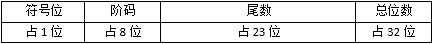
\includegraphics[width=4.51042in,height=0.45833in]{computerassets/48bfebac1b77986c4d0a719a76fe50e4.jpeg}
x,y的二进制表示如下: x=0100 0000 1110 1000 0000 0000 0000 0000 0000
y=1100 0010 0000 0100 0000 0000 0000 0000 0000
设x的阶码为jx,y的阶码为jy。 则{[}jx{]}移=1000 0001,{[}jy{]}移=1000
0100。
{[}∆E{]}补={[}jx-jy{]}补={[}jx{]}补-{[}jy{]}补={[}jx{]}移-{[}jy{]}移=1000
0001 -- 1000 0100 = 1111 1101。故本题选D。
\end{solution}
\question 浮点数加、减运算过程一般包括对阶、尾数运算、规格化、舍入和判溢出等步骤。设浮点数的阶码和尾数均采用补码表示,且位数分别为5位和7位(均含2位符号位)。

若有两个数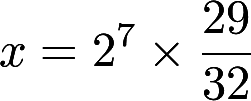
\includegraphics[width=0.90625in,height=0.35417in]{texmath/7c2c145Cdpi7B3507Dx3D25E75Ctimes5Cfrac7B297D7B327D}
,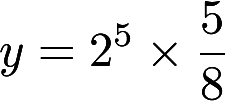
\includegraphics[width=0.81250in,height=0.36458in]{texmath/787c195Cdpi7B3507Dy3D25E55Ctimes5Cfrac7B57D7B87D},

则用浮点加法计算x+y的最终结果是( ~)
\par\fourch{00111 1100010}{00111 0100010}{01000 0010001}{\textcolor{red}{发生溢出}}
\begin{solution}首先,可将x、y分别记为00,111;00.11101和00,101;00.10100,然后根据浮点数的加法步骤进行计算。
第一步:对阶。x、y阶码相减,即00,111-00,101=00,111+11,011=00,010,当然这里就不用计算了,从题目给出的条件也可以看出,x的阶码比y的阶码大2。根据小阶向大阶看齐的原则,将Y的阶码加2,尾数右移2位,即y变成00,111;00.00101。
第二步:尾数相加。即00.11101+00.00101=01.00010,尾数相加结果符号位为01,故需进行右规。
第三步:规格化。将尾数右移1位,阶码加1,得x+y为01,000;00.10001,阶码符号位为01,说明发生溢出,且为正溢出。
【总结】 浮点数加/减运算步骤归纳如下:
(1)对阶。使两数的小数点位置对齐。对阶的规则是:小阶向大阶看齐。
(2)尾数求和或者求差。将对阶后的两尾数按定点加/减运算规则求和或者求差。
(3)规格化。为增加有效数字的位数,提高运算精度,必须将求和或求差后的尾数规格化。尾数一共可能出现以下6种情况。
① 00.1×× ××× ~ ~ ~ ② 11.0×× ××× ~ ③ 00.0×× ××× ~ ~ ~ ④ 11.1×× ××× ~ ⑤
01.××× ××× ~ ~ ~ ⑥ 10.××× ×××
其中,①和②符合规格化数的定义,无需规格化。③和④需要左规,次数不定。尾数每左移一位,阶码相应减1,直到成为规格化数为止。⑤和⑥其实在定点数中已经算是溢出了,但是在浮点数中,只能表示此时尾数的绝对值大于1,而并非真正的溢出。此时需要右规,次数最多1次。尾数每右移一位,阶码相应加1。
(4)舍入。为提高精度,要考虑尾数右移时丢失的数值位。常见的舍入法有``0舍1入''法和``恒置1''法。
当然,以上4个步骤完成后,还需要检查一下最后的结果是否溢出。由于浮点数的溢出完全是用阶码来判断的,假设阶码采用补码来表示,溢出就可以使用双符号位判断溢出的方式来判断此浮点数是否溢出,过程如下:
~ ~ ~ ~if(阶符==01) ~ ~ ~ ~ ~ ~ ~ ~上溢,需做中断处理; ~ ~ ~ ~else
~if(阶符==10) ~ ~ ~ ~ ~ ~ ~ ~下溢,按机器零处理; ~ ~ ~ ~else ~ ~ ~ ~
~ ~ ~ ~结果正确; 以上过程为完整的浮点数加/减运算过程。
\end{solution}
